\documentclass[12pt]{article}

\usepackage[spanish]{babel}
\usepackage[margin = 2.54cm]{geometry}
\usepackage[dvipsnames]{xcolor}
\usepackage{array, amssymb, amsthm, enumitem, float, graphicx, mathtools, hyperref}
\usepackage[backend = biber, style = IEEE, sortcites]{biblatex}

\addbibresource{referencias.bib}

\title{
	\textbf{Anteproyecto Trabajo Fin de Grado}
}

\author{
	Pablo García García\\
	{\small \href{mailto:pablo.ggarcia@edu.uah.es}{\texttt{pablo.ggarcia@edu.uah.es}}}
}

\date{
	\today
}

\hypersetup{
	pdftitle={Anteproyecto}, 
	pdfauthor={Pablo García García}, 
	pdfsubject={Trabajo de Fin de Grado}, 
	pdfcenterwindow, 
	pdfnewwindow=true, 
	pdfkeywords={}, 
	bookmarksopen=true 
}

\begin{document}
	
	\maketitle
	
	\noindent \textbf{Título}: Estudio de técnicas de visión e inteligencia artificial aplicadas a un caso práctico\\
	\textbf{Autor}: Pablo García García\\
	\textbf{Tutor}: Adrián Domínguez Díaz\\
	\textbf{Titulación}: Grado en Ingeniería Informática (G781)\\
	
	\section{Introducción}
	
		A día de hoy es complicado encontrar una persona joven o adulta que, al menos, no haya escuchado el término de \textit{Inteligencia Artificial}. Aunque actualmente mucha gente no es capaz de asignarle una definición formal y precisa aceptada por todos, podríamos entenderla como un software capaz de procesar información y razonar sobre esta con rasgos propios de un humano, como podrían ser el aprendizaje o el razonamiento entre otros. Aquellos más informados en el asunto, habrán oído hablar de ciertos modelos un tanto polémicos debido a la repercusión que han tenido sus sorprendentes respuestas, como por ejemplo, ChatGPT, GitHub Copilot, DALL-E, Midjourney, entre otras \cite{ia}. Cada una de estas está enfocado a ciertas tareas como, procesamiento del lenguaje natural (NLP), generación de imágenes, generación de código... \\
		
		Con los ejemplos mostrados previamente podemos darnos cuenta de que la inteligencia artificial no está enfocada a una única tarea, si no que dentro de esta existen diferentes sectores que nos permiten ayudar a resolver tareas muy complejas de diferente índole. El trabajo que se presenta, se enfocará en un sector de la inteligencia artificial, en concreto el de la visión artificial, en el que se pueden realizar gran cantidad de tareas en las que imágenes y vídeos estén involucrados. Se abordará el estudio de diferentes tecnologías y métodos relacionados con este campo, así como aplicaciones prácticas del mismo. \\
		
		Por otro lado, para ilustrar de dónde viene la idea práctica de este proyecto, hablaremos sobre la compañía Niantic, fundada en 2010 por John Hanke como parte de una \textit{startup} de Google, con la idea de desarrollar juegos para dispositivos móviles basados en mapas de la vida real. Algunas de las creaciones más conocidas de esta empresa fueron los juegos \textit{Ingress} (2012), y \textit{Pokémon GO} (2016) \cite{niantic}. Una de las herramientas creadas por esta empresa es Niantic Lightship, que permite a desarrolladores de juegos móviles en Unity, integrar realidad aumentada (AR) y mapas con puntos de interés basados en la ubicación en el mundo real del jugador \cite{lightship}. \\
		
		Centrándonos un poco más en este tema de puntos de interés en mapas del mundo, algunos ejemplos como podrían ser estatuas, museos, iglesias, parques, o cualquier punto que una persona local sepa que un turista no debería marcharse de dicho lugar sin visitar. Como es evidente, para Niantic sería imposible \textit{mapear} todo el mundo con estos puntos de interés, por lo que en 2019 lanzó la plataforma Niantic Wayfarer \cite{wayfarer}, donde usuarios experimentados de sus juegos pueden realizar propuestas de estos puntos de interés, mientras que a la vez, valoran las del resto de usuarios. \\
		
		Pasados cuatro años desde su lanzamiento, la comunidad notifica problemas de ``atasco'' del sistema, debido al reducido número de valoradores, y el enorme número de propuestas. Tras estas quejas de la comunidad, nace la idea final de este proyecto, el estudio y evaluación de diferentes técnicas de visión e inteligencia artificial para poder desarrollar un pequeño prototipo capaz de automatizar parte de la evaluación de ciertos conjuntos de propuestas, de forma que sirviese como iniciativa a la empresa para crear un sistema robusto que pudiese realizar de manera automática este trabajo para todo tipo de propuestas. 
	
	\section{Objetivos y campo de aplicación}
	
		Teniendo en cuenta un punto de vista más teórico, y más adelante uno ligeramente más práctico, algunos de los objetivos del proyecto a considerar serían los siguientes: 
		
		\begin{itemize}
			\item Investigación, aprendizaje, y explicación de diferentes técnicas y algoritmos de inteligencia y visión artificial para trabajar con imágenes, así como diferentes tecnologías a utilizar, y ámbitos en las que aplicarlas. 
			
			\item Con los aspectos teóricos investigados, aplicando algún lenguaje de programación y sus librerías, llevarlos a la práctica para realizar un pequeño prototipo que sea capaz de \textbf{automatizar alguna de las etapas de valoración} de una propuesta en la plataforma Wayfarer, entre las que podrían estar: 
			
			\begin{itemize}
				\item Clasificación de una imagen, en función del objeto que aparezca en esta para determinar si la propuesta debería ser elegible o no. 
				
				\item Dada una imagen, y otro conjunto de imágenes, detectar si el objeto que aparece en la primera, vuelve a aparecer en alguna del conjunto dado, para poder determinar si la propuesta es un duplicado, es decir, que el usuario solicitó algo que fue aprobado previamente. 
				
				\item Dada una imagen, detectar si esta forma parte de una imagen esférica de Google Street View, para comprobar si las coordenadas proporcionadas por el jugador son correctas. 
			\end{itemize}
			
			\item Fabricación de un ``\textit{dataset}'' o conjunto de datos propio basado en esta temática con el que poder evaluar los diferentes algoritmos o modelos que se propongan, para determinar la viabilidad de escalar el prototipo. 
		\end{itemize}
	
	\section{Descripción del trabajo}
	
		Este trabajo tendrá como objetivo final la realización de un pequeño prototipo de valorador automático (para ciertas etapas) de propuestas de Wayfarer, y para lograr esto podemos dividir las etapas del trabajo en las siguientes: 
		
		\begin{enumerate}[label = \textbf{\arabic*. }]
			\item \textbf{Estudio de técnicas de visión artificial}: para poder lograr los diferentes objetivos de este proyecto, lo primero que ha de hacerse es formarse, estudiar, y entender diferentes técnicas, algoritmos, y conceptos relacionados con el campo de la inteligencia y la visión artificial, pues sin una buena base de conocimientos teóricos será complicado obtener buenos resultados en la práctica. 
			
			\item \textbf{Investigación de tecnologías}: deberán estudiarse qué lenguajes o tecnologías son más convenientes para realizar este tipo de proyectos, así como si cada uno de estos posee librerías u herramientas que faciliten el trabajo, cuál es más rápido, cuál consigue mejores resultados, etc. 
			
			\item \textbf{Fabricación y tratamiento de los datos}: se fabricaría un \textit{dataset} propio recopilando imágenes (y coordenadas, si se decidiese llevar esta etapa de la valoración a cabo) con las que se pueda entrenar o evaluar a los diferentes algoritmos o modelos. También deberá hacerse un tratamiento previo de los datos para obtener unos resultados lo más óptimo posible. 
			
			\item \textbf{Desarrollo y pruebas}: una vez investigada y estudiada toda la teoría, sería el momento de llevarlo a la práctica en el/los lenguajes y tecnologías elegidas, trabajando con los datos y diferentes códigos que permitan entrenar modelos, supervisando el aprendizaje de estos. 
			
			\item \textbf{Comparativas}: podría llevarse a cabo una serie de comparativas variando el hardware, para estudiar como cambia el rendimiento en función de este. 
			
			\item \textbf{Documentación}: deberá quedar todo código comentado para que se pueda entender correctamente, así como la redacción de una memoria de proyecto donde se explique a fondo todos los contenidos teóricos y prácticos empleados. 
		\end{enumerate}
	
	\section{Metodología y plan del trabajo}
	
		En base a descripción del trabajo realizada en el punto anterior, podemos representar diferentes tareas y subtareas en un \textbf{diagrama de Gantt} realizado en Microsoft Project, con una duración estimada (podría llegar a extenderse debido a otros factores). El diagrama mostrado en la Figura \ref{fig:gantt} solo es una primera aproximación. Respecto a la metodología, una clásica y que se adapta al diagrama mostrado, es la \textbf{metodología en cascada}. Consiste en dividir el proyecto en etapas secuenciales, y antes de pasar de una a otra, hacer una revisión al finalizar cada una. 
		
		\begin{figure}[H]
			\centering
			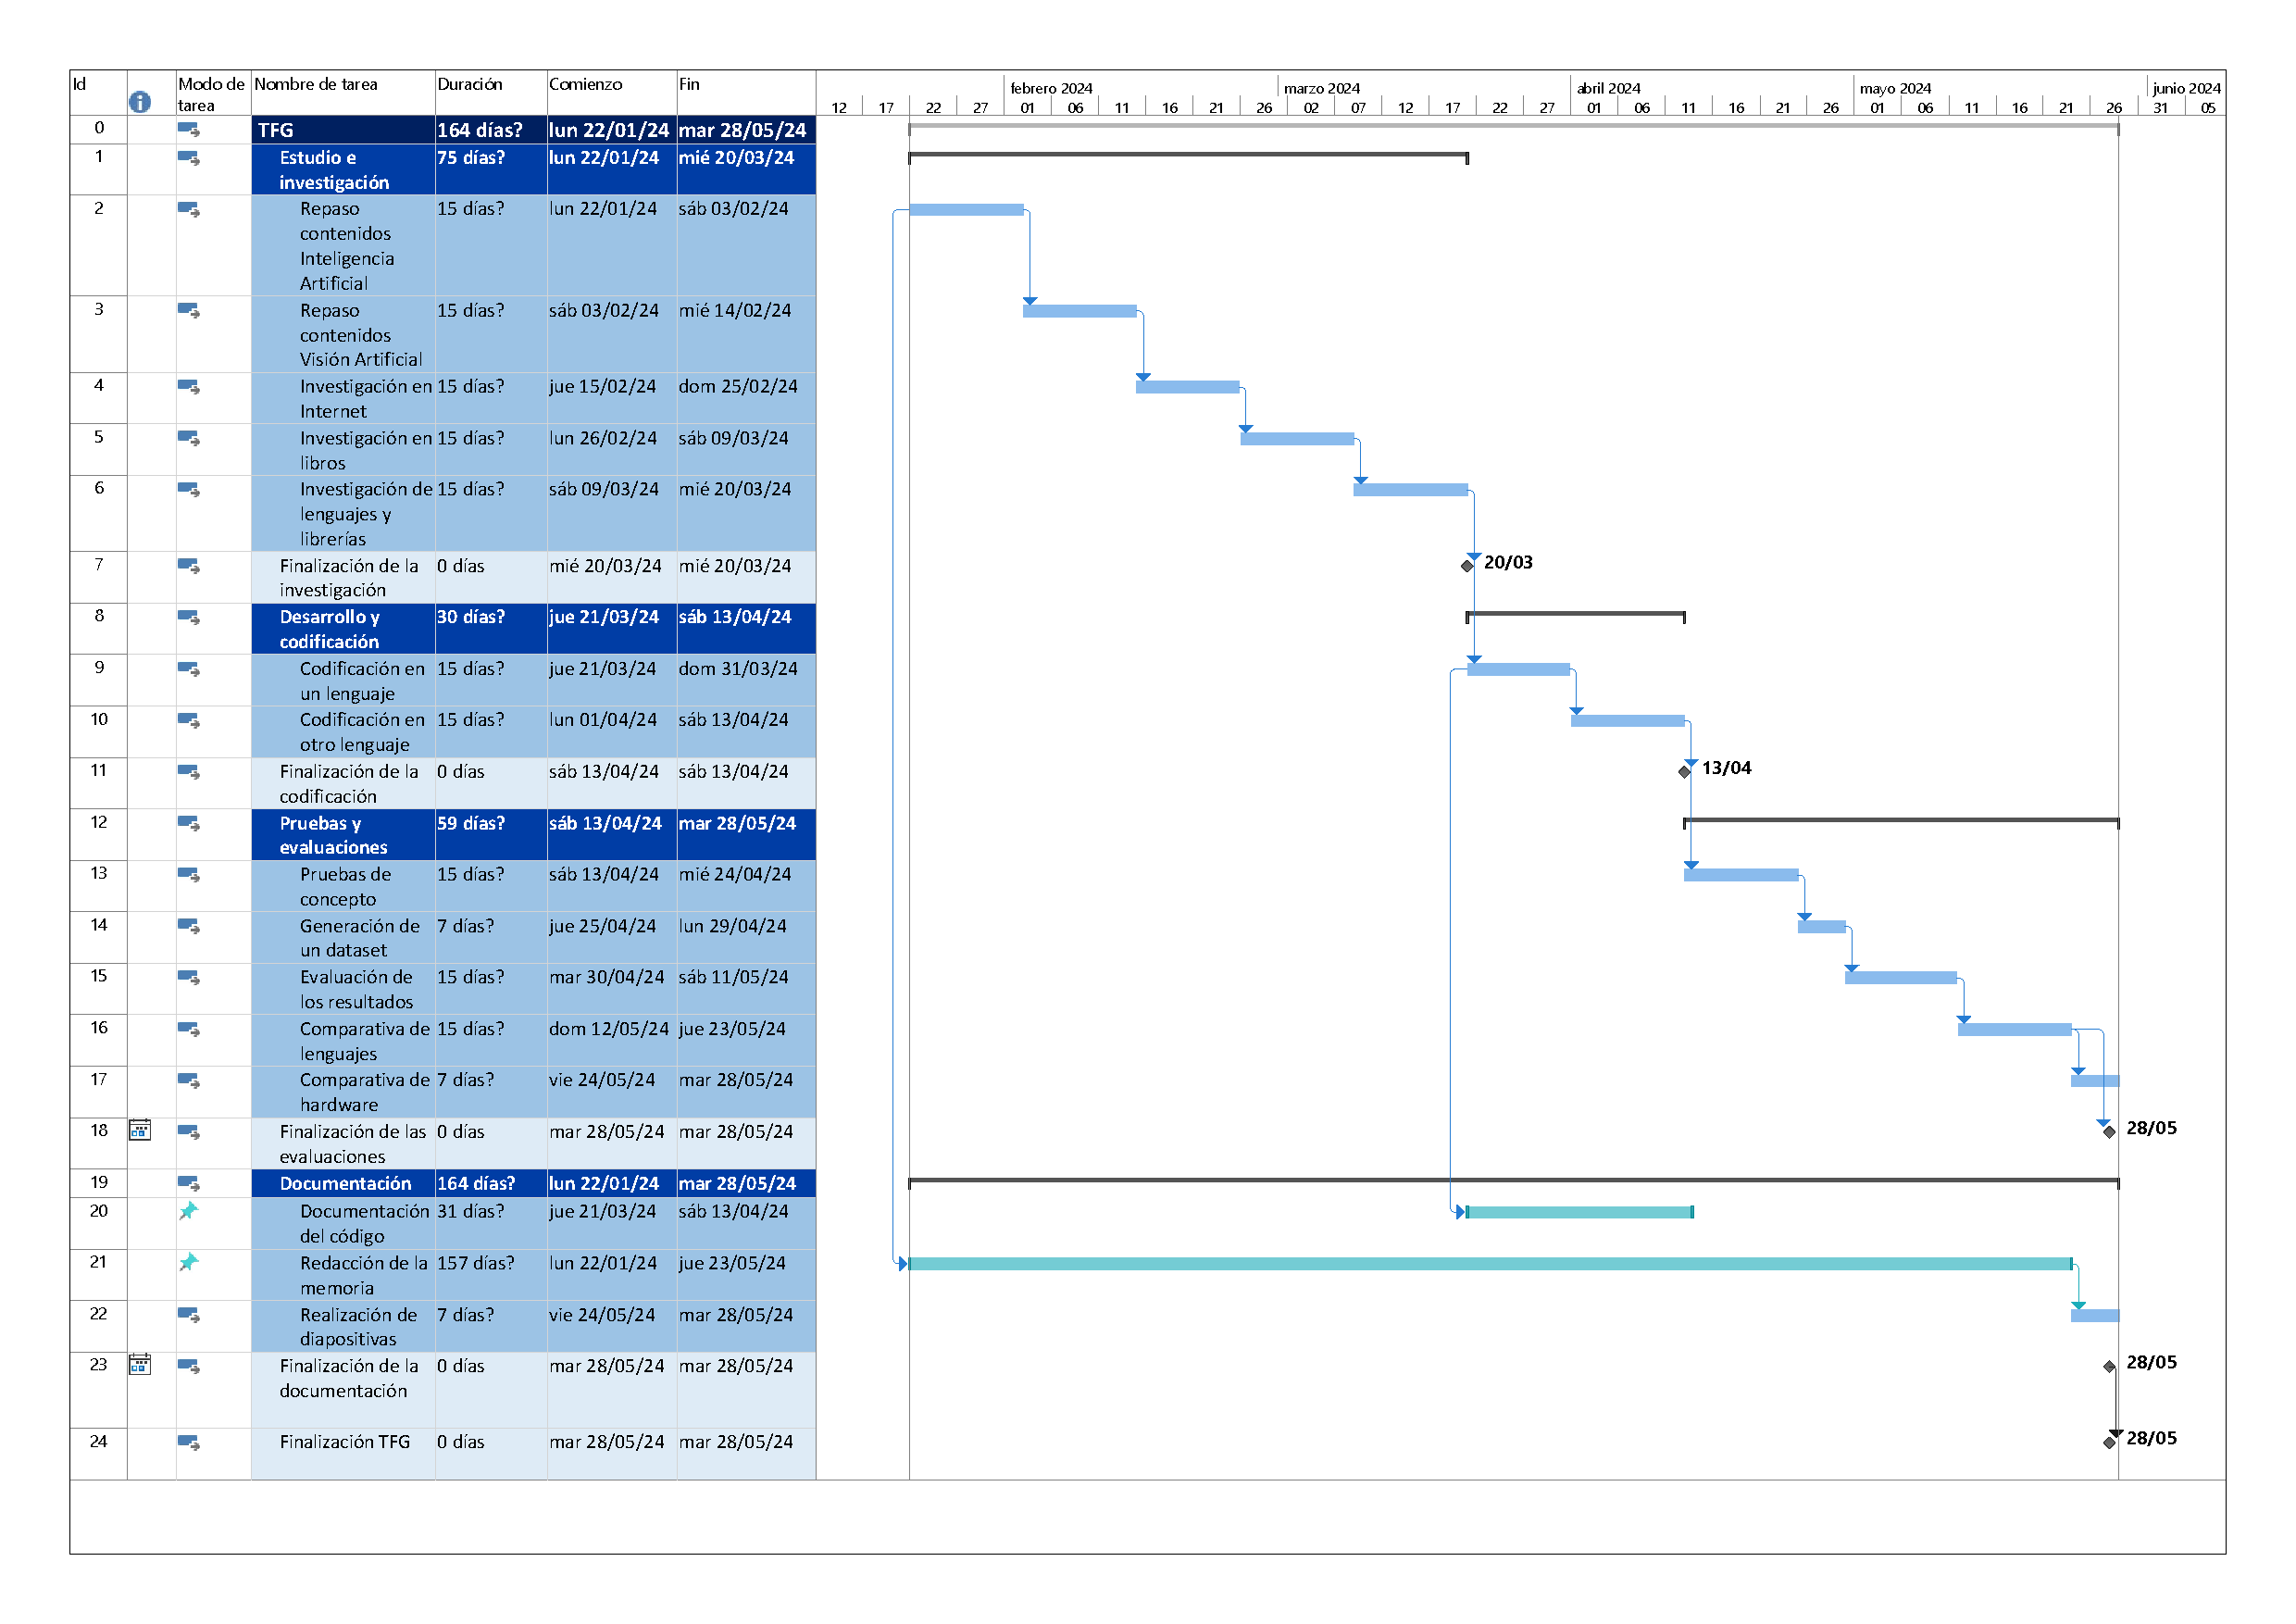
\includegraphics[scale = 0.4]{gantt}
			\caption{Diagrama de Gantt}
			\label{fig:gantt}
		\end{figure}
	
	\section{Medios}
	
		En respecto al material que será empleado, se disponen de los siguientes elementos, aunque no supondría un problema añadir más a futuro. 
		
		\begin{itemize}
			\item Un PC con conexión a Internet para poder realizar las investigaciones pertinentes, y componentes mínimamente capaces de trabajar con algoritmos que demanden una gran capacidad de cómputo. 
			
			\begin{itemize}
				\item Intel Core i7--8700
				\item NVIDIA GeForce GTX 1060 6GB
				\item 32GB RAM
			\end{itemize}
			
			\item Entornos de desarrollo, lenguajes, y librerías de uso libre. 
			
			\item En caso de necesitarse, entornos de desarrollo, lenguajes, servicios de computación, y librerías de pago, por ejemplo, licencia de MATLAB o de Microsoft Azure de la Universidad de Alcalá. 
			
			\item Un sistema de composición de textos de uso libre, como \LaTeX{}, para la realización de la memoria del proyecto e informes que procedan. 
			
			\item Un software de administración de proyectos, como Microsoft Project (licencia de la Universidad de Alcalá), para el desarrollo del diagrama de Gantt, y una correcta gestión del proyecto. 
			
			\item Cuenta con acceso habilitado a Wayfarer, para un mejor entendimiento del sistema y recolección de datos. 
		\end{itemize}
	
	\printbibliography

\end{document}          
